\documentclass[9pt, compress, xcolor=table]{beamer}


\usetheme{m}

\usepackage{amsmath,amssymb,amsthm}
\usepackage{latexsym}
\usepackage{booktabs}
\usepackage[scale=2]{ccicons}
\usepackage{minted}
\usepackage[english, russian]{babel}
\usepackage{graphicx}
\usepackage{xcolor}
\usepackage{euscript}
% \DeclareMathOperator{\arctg}{arctg}
\usepackage{tabu} % https://ru.sharelatex.com/learn/Tables
\DeclareGraphicsExtensions{.pdf,.jpg,.png}
\graphicspath{{../images/}{./images/}}

\colorlet{Mycolor1}{green!50!blue!50!}
\DeclareMathOperator{\Ima}{Im}
\usemintedstyle{trac}

\title{Физические принципы оптической микроскопии сверхвысокого разрешения}
\subtitle{осенний семестр, 2015}
\author{ассистент, к.ф.-м.н. Шутова О.А.}
\institute{МГУ им. М.В. Ломоносова, физический факультет}

\begin{document}

\maketitle

\plain{}{Лекция 11. Обзор дальнепольных методов микроскопии сверхразрешения}

\begin{frame}{Основные методы}

\textcolor{red!50!black}{\textbf{Дальнепольная микроскопия сверхразрешения}} (во всё большем количестве статей ее называт \textcolor{red!50!black}{\textbf{наноскопией}}) - это три семейства методов. Превышение дифракционного предела, достижимое с помощью этих методов составляет до \textcolor{red!50!black}{\textbf{$\lambda/100$}}, т.е. превосходит предел Аббе на порядок.
\begin{columns}[c]
\column{4cm}
\begin{center}
\textcolor{red!50!black}{\textbf{Сильно-сфокусированные пучки:}}

\textbf{STED} 

{\small stimulated emission depletion} 

\textbf{GSD} 

{\small ground state depletion}

\textbf{4 $\pi$ - микроскопия}

\textbf{RESOLFT}

{\small reversible saturable optical fluorescence transitions microscopy}

\textbf{...}
\end{center}
\column{4cm}
\begin{center}
\textcolor{red!50!black}{\textbf{Модуляция накачки и/или возбуждающего поля:}}

\textbf{SIM}  

{\small structured illumination microscopy}

\textbf{PEM}

{\small patterned excitation microscopy}

\textbf{SW}

{\small standing wave microscopy}

\textbf{SMI}  

{\small spatially modulated illumination microscopy}
\end{center}
\column{4cm}
\begin{center}
\textcolor{red!50!black}{\textbf{Локализационная микроскопия:}}

\textbf{SALM} 

{\small spectrally assigned localization microscopy}

\textbf{PALM}

{\small photoactivable localization microscopy}

\textbf{STORM}

{\small stochastic optical reconstruction}

\textbf{...}
\end{center}

\end{columns}

\end{frame}

\begin{frame}{Общие принципы}

\textcolor{red!50!black}{\textbf{Теория разрешения оптического прибора по Аббе}} предполагала, что набор одновременно излучающих/поглощающих/ рассеивающих объектов, находящихся в плоскости объекта, по излучению в плоскости изображения должен быть максимально точно восстановлен. 

Волновая природа света указывает на верхний предел разрешения в такой системе. \textcolor{red!50!black}{\textbf{Методы ближнепольной микроскопии}} основаны на различных способах не потерять неоднородные волны, несущие информацию о высоких пространственных частотах и отсутствующие в обычном оптическом приборе из-за того, что локализуются очень близко к поверхности объекта.

\textcolor{red!50!black}{\textbf{Методы дальнепольной микроскопии}} основаны на принципиально иной идее: на введении в систему дополнительных параметров управления, которые позволили бы нам не преодолеть этот предел, а по сути обойти его. Например, можно заставить объекты излучать не одновременно, а строго по очереди по известному нам временному закону. Развитие этих методов остро связано с успехами в области синтеза т.н. \textcolor{red!50!black}{\textbf{фотоактивируемых белков}}.  


\end{frame}

\begin{frame}{Литература}

\begin{itemize}
\item Работы группы \textcolor{red!50!black}{\textbf{Штефана Хелля}} (Stefan W. Hell, университет Макса Планка, STED  и др.) (нобелевская премия по химии, 2013): сайт 4pi.de 
\item Работы \textcolor{red!50!black}{\textbf{Кристофа Кремера}} (Christoph Cremer, университет Гайдельберга): (1) книга \textbf{Optics Far Beyond Diffraction Limit}, Springer, 2012; (2)  обзор \textbf{Resolution enhancement technics in microscopy}, EPJ D, 2013, p.283-344
\item Работы \textcolor{red!50!black}{\textbf{Гаральда Хесса}} (Harald Hess, Исследовательский центр HHMI, Вирджиния, PALM): сайт janelia.org (там же Эрик Бетциг, соавтор по нобелевской премии)
\item Работы \textcolor{red!50!black}{\textbf{Сяо Вэй Чжун}} (Xiaowei Zhuang, Гарвард, STORM): сайт zhuang.harvard.edu
\end{itemize}

\end{frame}

\plain{}{Предварительные замечания}
\begin{frame}{Функция рассеяния точки}

\begin{columns}[c]
\column{2.2in}

{\small Точечный диполь, расположенный на оси оптической системы и произвольно
ориентированный относительно нее в плоскости изображения представляет собой трехмерное
распределение поля, свойства которого, а также направление вектора поля, зависят от параметров
оптической системы. Передаточная функция ОС называется \textcolor{red!50!black}{\textbf{ функцией рассеяния точки (point spread function, PSF)}}}

\column{2.2in}
\begin{center}
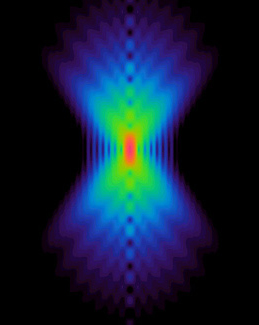
\includegraphics[width=4cm]{fig4_24}
\end{center}
\end{columns}

Для описания отклика системы мы введем понятие объема наблюдения:

\begin{equation*}
V_{obs}= \frac{4\pi}{3}PSF_{FWHMx}PSF_{FWHMy}PSF_{FWHMz}
\end{equation*}

{\small Таким образом, для описания передачи изображения трехмерных объектов нам необходимо ввести в дополнение к классическому понятию разрешающей способности, разрешающую способность в осевом направлении.}
\end{frame}

\begin{frame}{Задание ОС}

\begin{center}
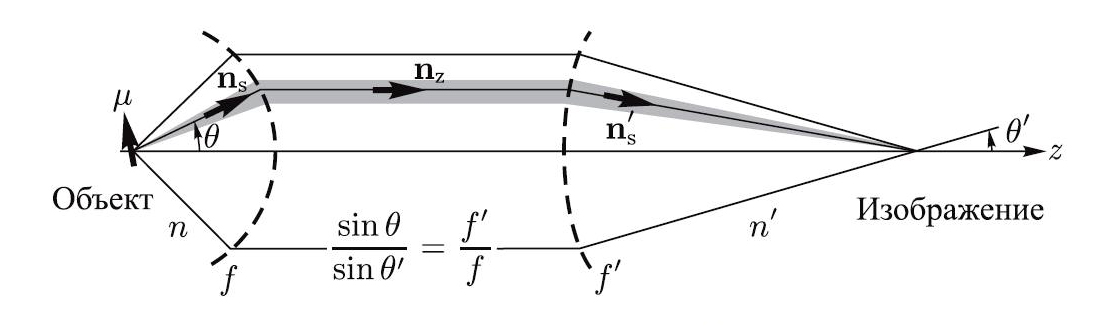
\includegraphics[width=0.9\textwidth]{fig4_01}
\end{center}

{\small Введем параметры оптической системы: числовую апертуру и коэффициент увеличения
(поперечный):}
\begin{equation*}
NA = n \sin \theta_{max},\qquad M = \frac{n}{n'} \frac{f'}{f}
\end{equation*}

{\small Ширина (диск Эйри) и глубина поля:}

\begin{equation*}
\Delta x = 0.6098 \frac{M \lambda}{NA}\qquad \Delta z = 2 n'\frac{M^2 \lambda}{NA^2}
\end{equation*}

{\small Характерные значения: для $NA = 1.4$, $M = 60\times$, $\lambda = 500$ нм глубина и ширина
поля $\Delta x = 13\,\mu m$, $\Delta z = 1,8\,mm$. Глубина поля больше, чем длина приблизительно в $M/NA$ раз.}
\end{frame}

\begin{frame}{ФРТ диполей, ориентированных вдоль и поперек ООС}

{\small Параксиальная функция рассеяния точки для
диполя, ориентированного вдоль оси $x$:}
\begin{equation*}
\lim_{\theta_{max} \ll \pi/2} |\vec E(x,y,z =0)|^2
= \frac{\pi^4}{\epsilon_0^2 n n'} \frac{\mu_x^2}{\lambda^6} \frac{NA^4}{M^2}
\left[2 \frac{J_1 (2 \pi \tilde{\rho})}{2 \pi \tilde{\rho}}\right]^2,
\quad \tilde{\rho} = \frac{NA}{M}\frac{\rho}{\lambda}
\end{equation*}

\begin{equation*}
\lim_{\theta_{max} \ll \pi/2} |\vec E(x = 0, y = 0, z)|^2 = \frac{\pi^4}{\epsilon_0^2 n n'} \frac{\mu_x^2}{\lambda^6}
\frac{NA^4}{M^2}\left[\frac{\sin (\pi \tilde{z})}{\pi \tilde{z}}\right]^2, \quad \tilde{z} = \frac{NA^2 z}{2n'M^2 \lambda}
\end{equation*}

{\small Параксиальная функция рассеяния точки для
диполя, ориентированного вдоль оси $z$:}
\begin{equation*}
\lim_{\theta_{max} \ll \pi/2} |\vec E(x,y,z =0)|^2 = \frac{\pi^4}{\epsilon_0^2 n/3 n'} \frac{\mu_z^2}{\lambda^6} \frac{NA^6}{M^2}
\left[2 \frac{J_2 (2 \pi \tilde{\rho})}{2 \pi \tilde{\rho}}\right]^2
\end{equation*}
\begin{center}
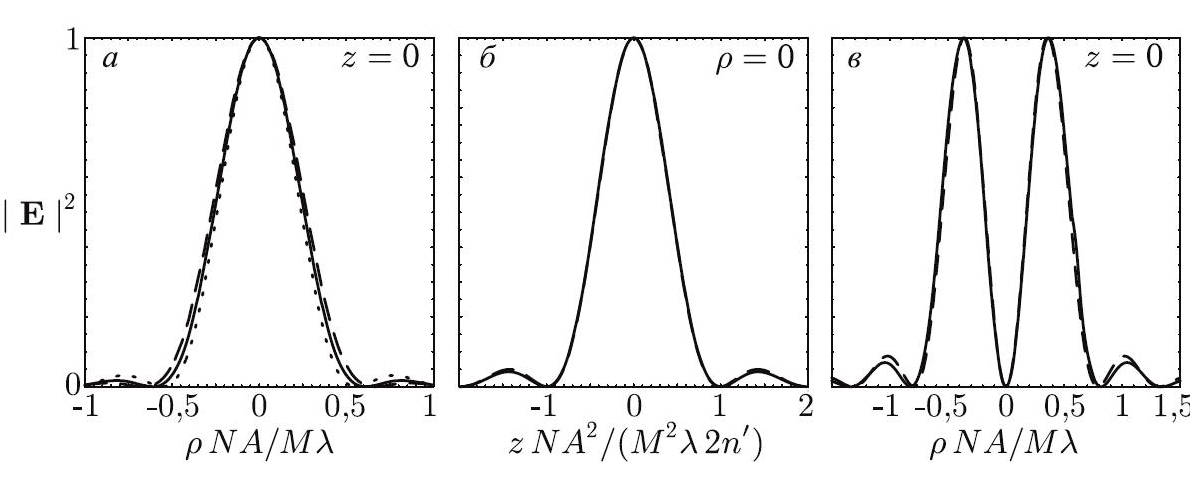
\includegraphics[width=0.6\textwidth]{fig4_02}
\end{center}

\end{frame}

\begin{frame}{Классический предел разрешения}

\begin{center}
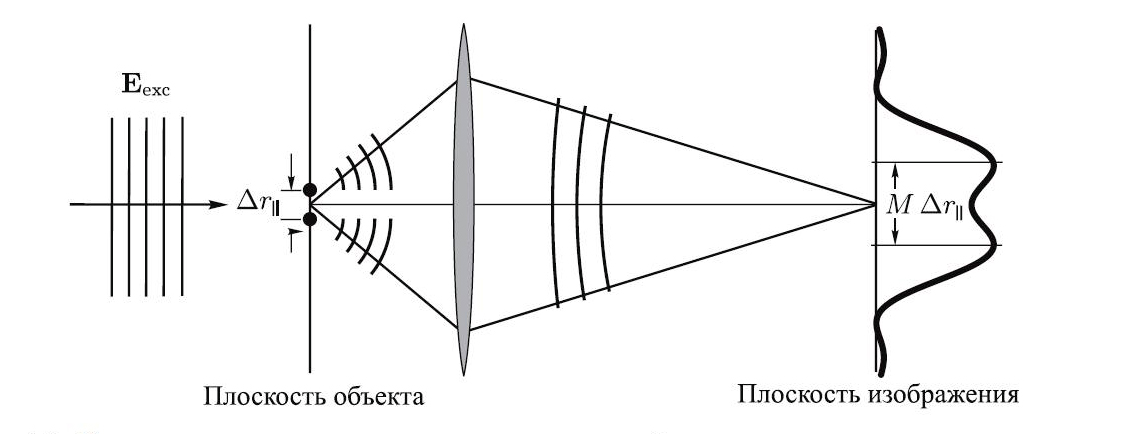
\includegraphics[width=6.5cm]{fig4_03}
\end{center}

{\scriptsize $\Delta k_{||} \Delta r_{||} \geq 1$: минимизируется это соотношение гауссовским
профилем поля (аналогично волновой функции в квантовой механике). Отсюда $ Min [r_{||}] =
\frac{\lambda}{2 \pi n}$ или $Min [r_{||}] = \frac{\lambda}{2 \pi NA}$}

\begin{equation*}
\boxed{
\textbf{Аббе (1873):}\qquad Min [r_{||}] = 0.6098\frac{\lambda}{NA}}
\end{equation*}
{\scriptsize Эта оценка в $3,8$ раз хуже, чем первая. Кроме того, она предполагает, что диполи
перпендикулярны ОС, что не всегда так. Она ухудшается также, если диполи не равны.}

\begin{center}
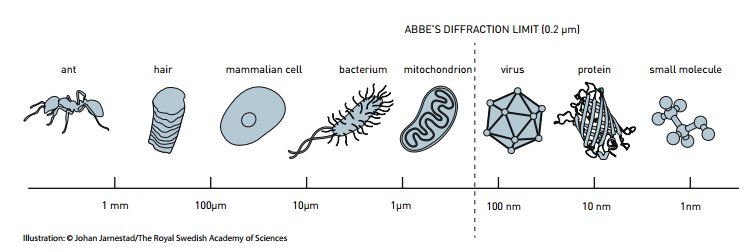
\includegraphics[width=0.7\textwidth]{ffm0}
\end{center}

\end{frame}
\begin{frame}{Поперечное разрешение}
\begin{center}
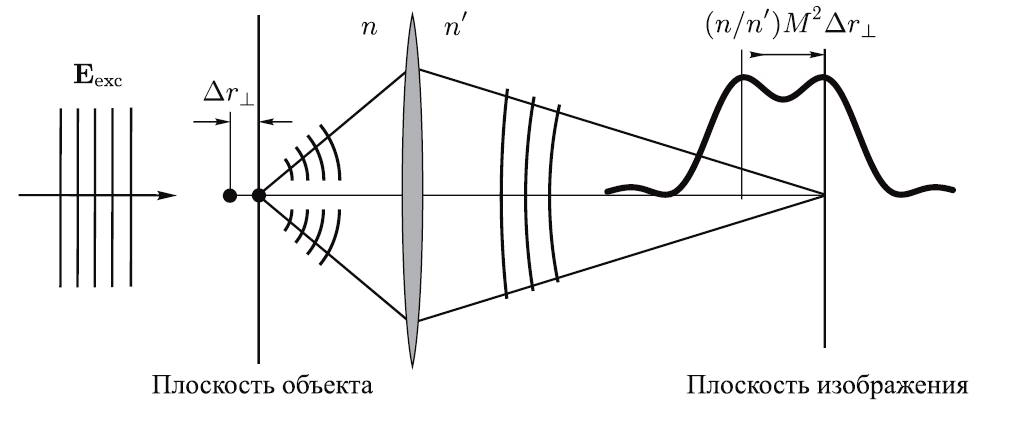
\includegraphics[width=7cm]{fig4_05}
\end{center}
{\small Если мы не будем осуществлять пространственную фильтрацию перед экраном, изображение будет предсталять интегральную величину, не зависящую от z (т.е. поперечное разрешение отсутствует).}
\begin{multline*}
s_2(z) \equiv \vec E(\rho = 0, z) E^{*}(\rho = 0, z) dA =\\=
\frac{\pi^4}{\epsilon_0^2 n n'} \frac{\mu_x^2 + \mu_y^2}{\lambda^6}
\frac{NA^4}{M^2}\left[\frac{\sin (\pi \tilde{z})}{\pi \tilde{z}}\right]^2 dA, \quad \tilde{z} =
\frac{NA^2 z}{2n'M^2 \lambda}
\end{multline*}
\begin{equation*}\boxed{
M_L = \frac{n}{n'} M^2\qquad Min[\Delta r_{\perp}] = 2\frac{n \lambda}{NA^2}}
\end{equation*}
{\small \textbf{Предварительное знание об ориентации диполей позволит нам эффективно увеличить пространственное разрешение ОС.}}
\end{frame}

\begin{frame}{Демонстрация возможностей осевого разрешения}

\begin{center}
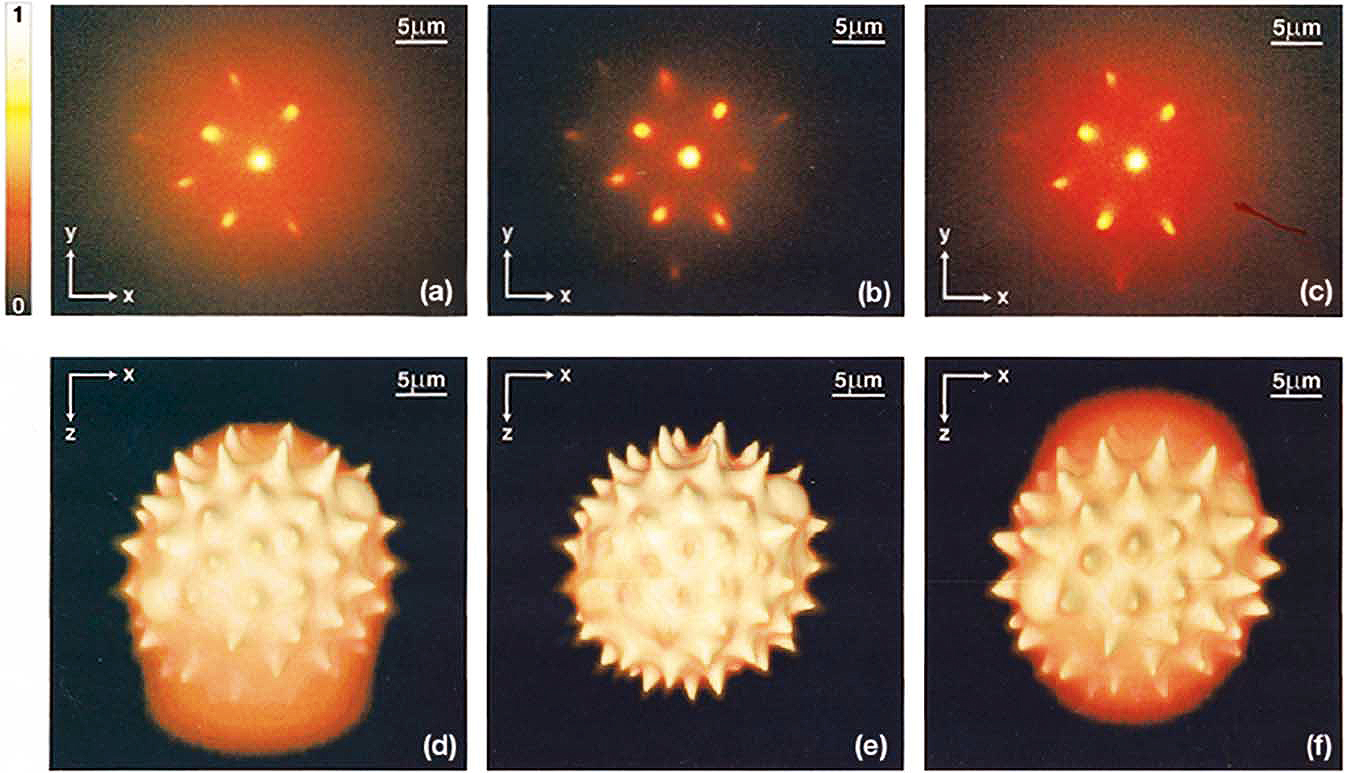
\includegraphics[width=9cm]{fig4_06}
\end{center}

{\small (a) MMM-6.4, (b) MMM-TMX-6.4, and (c) MMM-TMX-4.7. На (c) и (f) плотность фокусов такая же как в (a) и (d), но выше скорость. Time-multiplexed multifocal multiphoton microscope V. Andresen, A. Egner, and S. W. Hell, OPTICS LETTERS, Vol. 26, No. 2 (2001)}

Multifocal Multiphoton Microscopy (MMM) - это методика, как и STED и 4Pi, развивается в группе Штефана Хелля (Отделение Нанобиофотоники университита Макса Планка).

\end{frame}

\begin{frame}{Схема эксперимента}
\begin{columns}[c]
\column{6.5cm}
\begin{center}
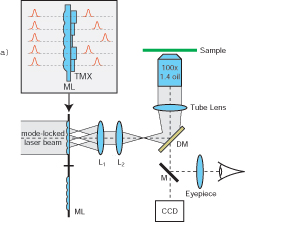
\includegraphics[width=0.9\textwidth]{MMM}
\end{center}
\column{6.5cm}
\begin{center}
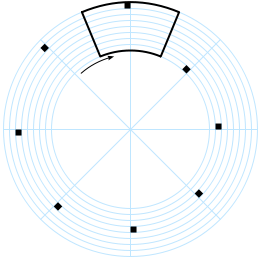
\includegraphics[width=0.7\textwidth]{MMM_0}
\end{center}
\end{columns}
В МММ используется Ti:Sa лазер (800 нм), излучение которого при помощи вращающегося набора микролинз, выстренных по спирали по принципу диска Нипкова, разделяется на 25-30 подпучков. Длина импульсов 130 фс, задержка 250, что гарантирует, что возбуждающие поля соседних подпучков не пересекаются во времени.
\end{frame}

\begin{frame}{Принцип селективного воздействия}

{\small Вообще любая предаврительная информация о свойствах среды (геометрическая, спектроскопическая и т.д.) может быть использована для повышения разрешающей способности. Причем не только в пассивном ключе, но и в плане управления откликом, т.н. \textcolor{red!50!black}{\textbf{инжеренрия ФРТ}}.}

\begin{center}
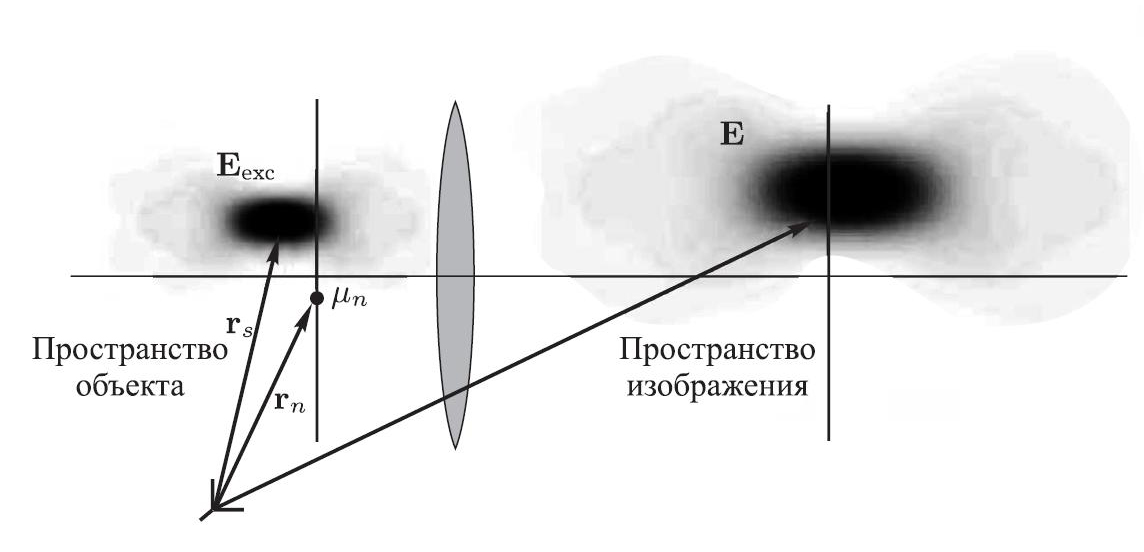
\includegraphics[width=7cm]{fig4_04}
\end{center}
\begin{multline*}
\vec \mu_n (\omega, 2\omega, .\,.\,.; \vec r_s, \vec r_n) = \\=\alpha (\omega) \vec E_{exc}
(\omega, \vec r_s - \vec r_n) + \beta (2\omega) \vec E_{exc} (\omega, \vec r_s - \vec
r_n)\vec E_{exc} (\omega, \vec r_s - \vec r_n) + .\,.\,.,
\end{multline*}
\begin{equation*}
\vec \mu_n (\omega, 2\omega, \ldots; \vec r_s, \vec r_n) = \vec \mu_n (\omega, \vec r_s, \vec r_n)
+ \vec \mu_n (2\omega, \vec r_s, \vec r_n) + \vec \mu_n (3\omega, \vec r_s, \vec r_n) + \ldots
\end{equation*}
\begin{equation*}
\vec E(\vec r, \vec r_n, \vec r_s; n\omega) = \frac{(n \omega)^2}{\epsilon_0 c^2} \overleftrightarrow{\vec G}_{PSF}(\vec r, \vec r_n, \vec r_s; n\omega)
\cdot \vec \mu_n (n\omega, \vec r_n, \vec r_s)
\end{equation*}

\end{frame}

\plain{}{Семейство 1: Сильно-сфокуcированные пучки}

\begin{frame}{4Pi-микроскопия}
\begin{center}
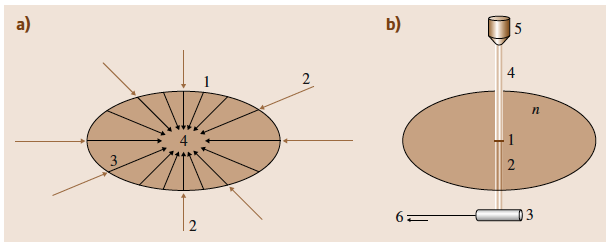
\includegraphics[width=0.9\textwidth]{ffm01}

Идея создания 4$\pi$ - микроскопии зародилась еще в 1970-х годах и базировалась на кардинальном влиянии на такой параметр системы как числовая апертура, стоящий в знаменателе предела Аббе. 4$\pi$ - означает освещение исследуемого объекта со всех сторон, т.е. со стороны телесного угла 4$\pi$ стерадиан.  

В чем-то идея родственна идее голографии (голо- с греч. \textit{целое}). Благодаря чему мы получаем 3D-изображение? Мы записываем разность фаз опроного и базового света, а она зависит от пространственных свойств. Вопрос в реализации.
\end{center}
\end{frame}

\begin{frame}{Реализация 4 Pi -микроскопии}
\begin{columns}[c]
\column{6cm}
\begin{center}
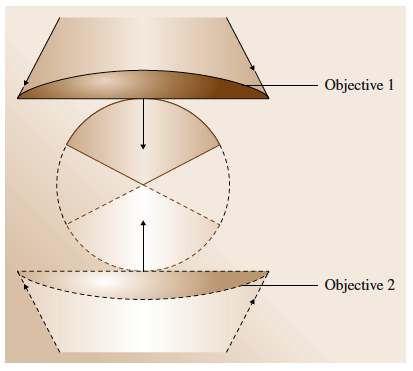
\includegraphics[width=0.9\textwidth]{ffm02}
\end{center}
{\small Если совместить идею 4Pi-микроскопии (в такой схеме достигается 2.7 $\pi$) с конфокальной и/или двухфотонной микроскопией, то можно достичь уменьшения объема исследования на порядок.}
\column{6.5cm}
\begin{center}
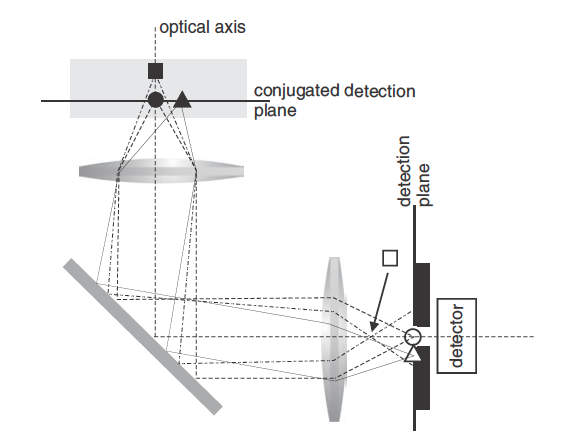
\includegraphics[width=0.85\textwidth]{ffm02a}

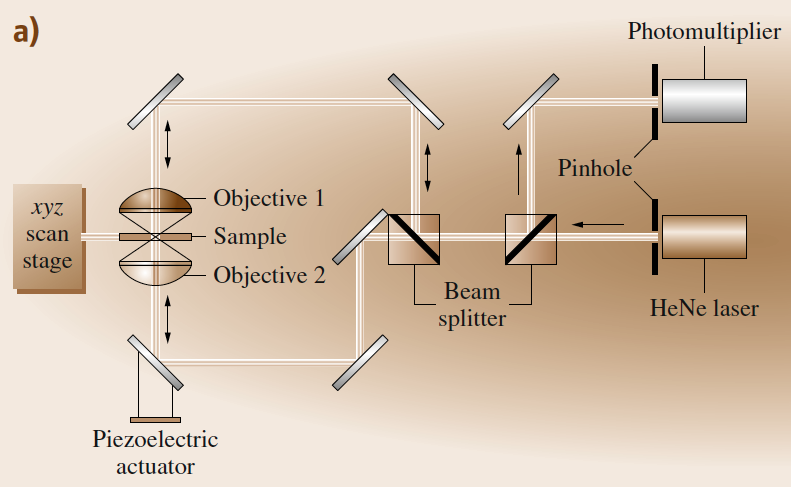
\includegraphics[width=0.85\textwidth]{ffm02b}
\end{center}
\end{columns}
\end{frame}

\begin{frame}{Возможные схемы}
\begin{columns}[c]
\column{6.3cm}
\begin{center}
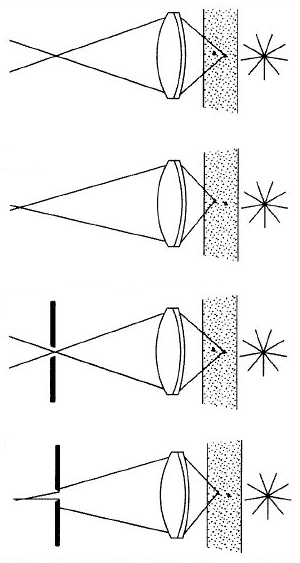
\includegraphics[width=0.7\textwidth]{fig4_08a}
\end{center}
\column{6.3cm}
\begin{center}
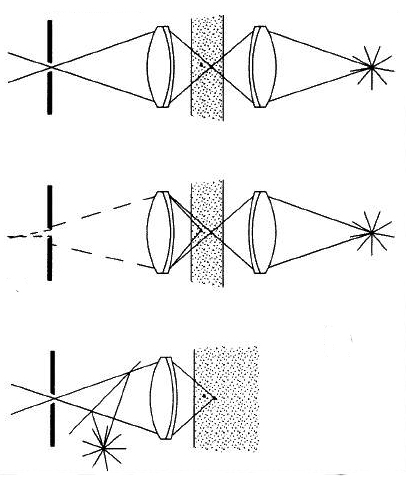
\includegraphics[width=0.8\textwidth]{fig4_08b}
\end{center}

{\small Вводя в систему возможность наклона предметной плоскости (т.н. микроосевая томография), 4Pi+МОТ уменьшаем $V_{obs}$
в 40 раз по сравнению с конфокальной}
\end{columns}
\end{frame}

\begin{frame}{Совмещение 4Pi и нелинейного возбуждения}
\begin{columns}[c]
\column{8cm}
\begin{center}
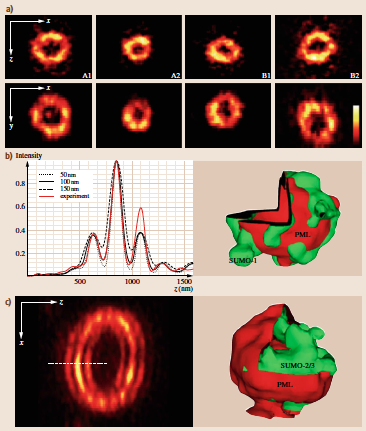
\includegraphics[width=0.9\textwidth]{ffm08}
\end{center}
\column{4cm}
\begin{center}
{\small Тело белка PML (промиелоцитарного лейкоза) человека в ядре клетки U2OS (остеосаркома) и HeLa клеток. 

Диаметр вдоль оси $\approx 600$ нм, толщина оболочек $100$ нм.

Справа снизу - реконструкция. PML - белок раковой клетки. SUMO - убиквитино-подобный белок, способный к протеолизу. Дополнительно применялись методы фурье-фильтрации.}
\end{center}
\end{columns}
\end{frame}


\begin{frame}{STED-микроскопия}

STED - stimulated emission depression. Идея: погасить излучатели, находящиеся на периферии фокального пятна, тем самым его сузив.
\begin{equation*}
\gamma_e (\vec r) = \sigma I_e(\vec r) / \hbar \omega_0\qquad\text{- скорость поглощения}
\end{equation*}
\begin{equation*}
\frac{\gamma_r}{\gamma_r + \gamma_d}\qquad\text{- вероятность испускания фотона флуоресценции, где}
\end{equation*}
\begin{equation*}
\gamma_d (\vec r) = \sigma I_d(\vec r) / \hbar \omega_0\qquad\text{- скорость вынужденного испускания}
\end{equation*}
\begin{equation*}
\gamma_{fl} (\vec r) = \gamma_e \frac{\gamma_r}{\gamma_r + \gamma_d (\vec r)} = \frac{\sigma}{\hbar \omega_0}
\frac{I_e (\vec r)}{1 + d_p (\vec r)}\qquad\text{- скорость актов флуоресценции}
\end{equation*}
\begin{equation*}
d_p(\vec r) \equiv \frac{\sigma}{\hbar \omega_0 \gamma_r} I_d(\vec r)\qquad\text{- параметр истощения излучательной способности}
\end{equation*}
\begin{equation*}
\boxed{Min[\Delta r_{||}] \approx 0.6098 \frac{\lambda}{NA \sqrt{1 + d_p}}}
\end{equation*}
\begin{center}
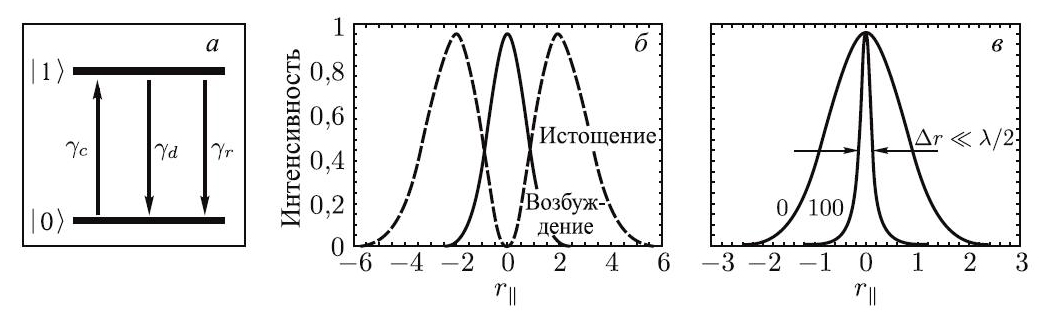
\includegraphics[width=10cm]{fig4_07f}
\end{center}

\end{frame}

\begin{frame}{Схема эксперимента}
\begin{columns}[c] \column{4cm}
\begin{center}
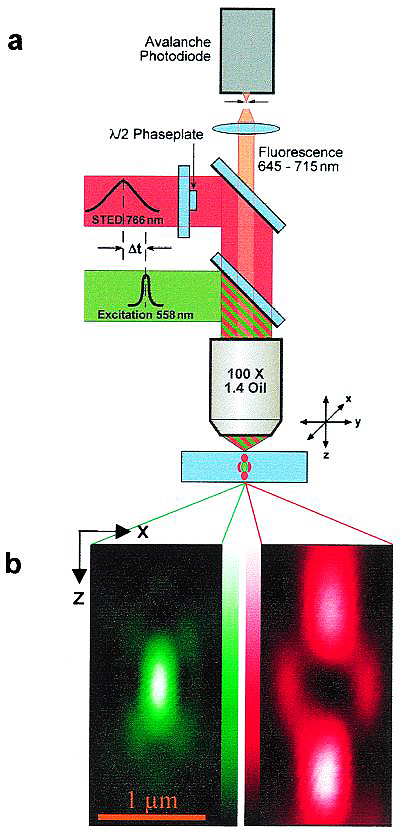
\includegraphics[width=0.8\textwidth]{fig4_07b}
\end{center}
\column{8cm}
\begin{center}
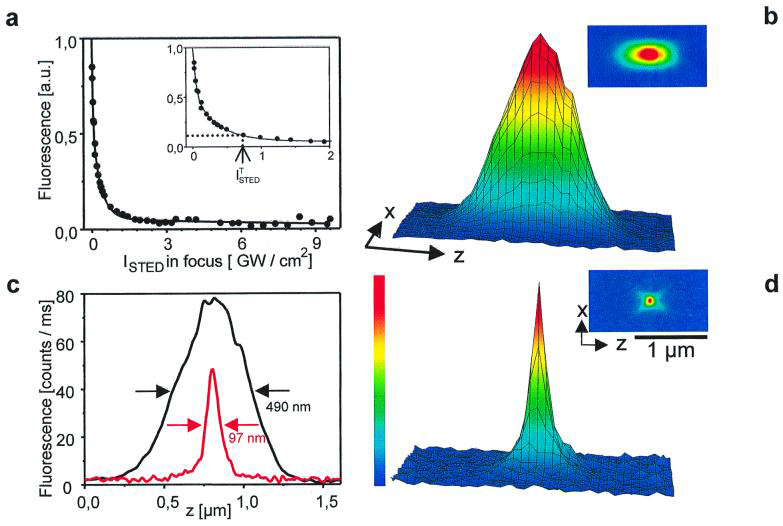
\includegraphics[width=0.7\textwidth]{fig4_07a}

\begin{center}
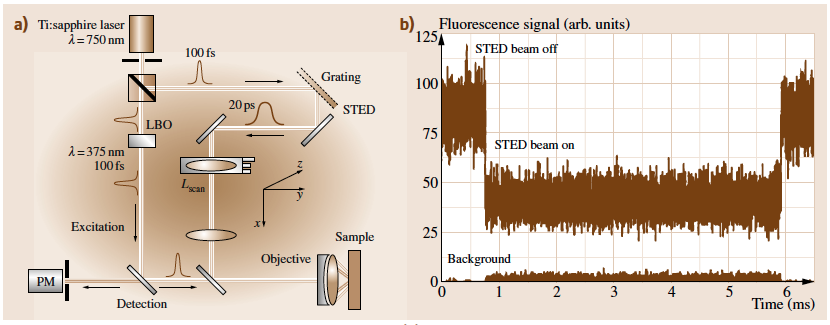
\includegraphics[width=0.9\textwidth]{ffm03}
\end{center}
{\small Возбуждение - 375 нм, сигнал в диапазоне 600-700 нм. По интенсинвости теряем вдвое, значит доля темных к светлым $1-1/\sqrt{2}\approx 1.6$ }
\end{center}

\end{columns}

\end{frame}

\begin{frame}{Сочетание с модуляционными техниками}

Возможно сочетание STED с модуляционными техниками, о которых мы говорили ранее в связи с ближнепольной микроскопией.

K. Fujita et al. High-Resolution Confocal Microscopy by Saturated Excitation of Fluorescence", PRL 99, 228105 (2007)
\begin{columns}[c] 
\column{6cm}
\begin{center}
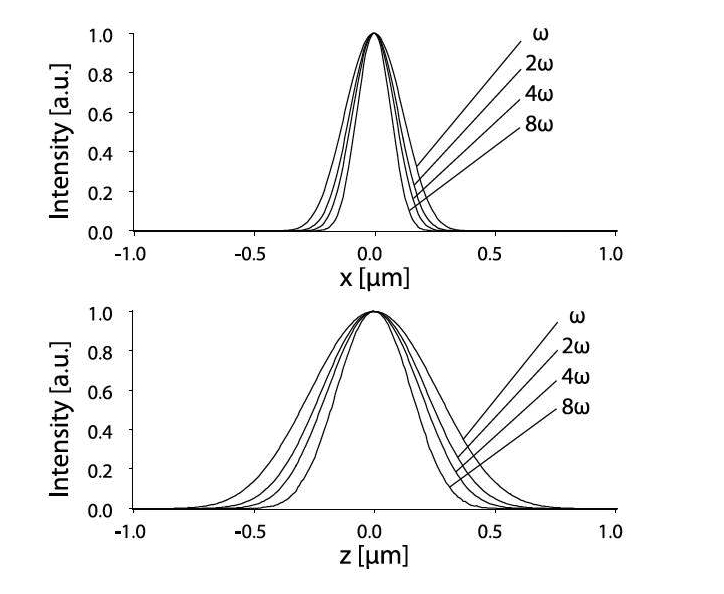
\includegraphics[width=6cm]{fig4_07e}
\end{center}

\column{6cm}
\begin{center}
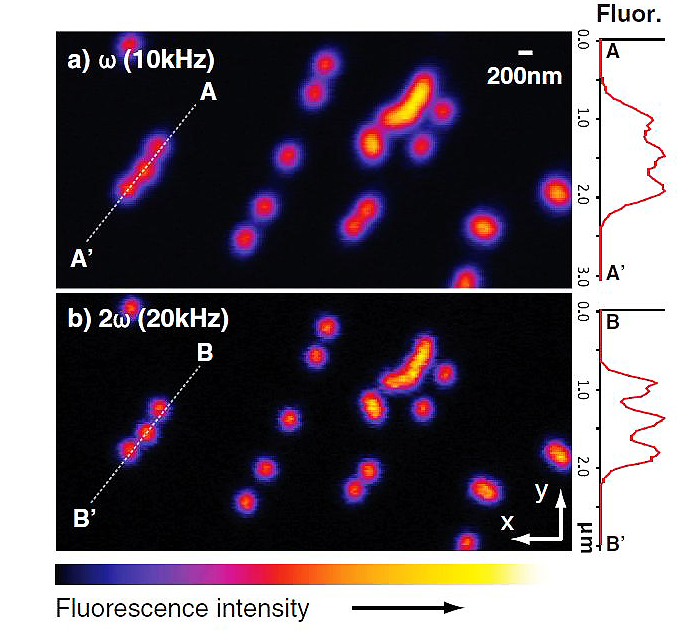
\includegraphics[width=6cm]{fig4_07c}
\end{center}
\end{columns}
Коммерчески доступный STED-микроскоп позволяет получить разрешение 70-80 нм (по данным 2012 г.).
\end{frame}

\plain{}{Исследование квантовых точек с помощью STED, 2015}

\begin{frame}{Свойства квантовых точек}
\begin{center}
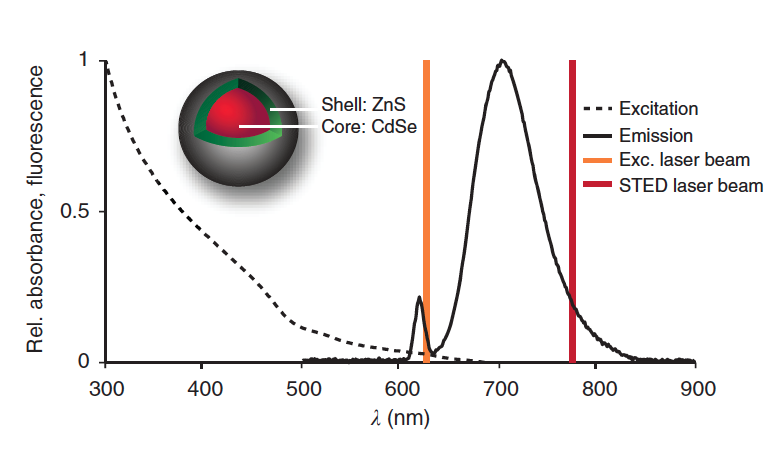
\includegraphics[width=0.6\textwidth]{ffm22}
\end{center}

S.Hell et al. Nature communications, 2015. Коммерчески досутпная квантовая точка QDot705, Life Technologies GmbH, Germany

{\small STED-микроскопия на основе флуоресцентных молекул широко развилась и была протестирована на большинстве классов флуорофоров. Проблема флуоресцентных молекул состоит в выгорании. Квантовые точки (вдали от промежуточных переходов в метастабильные темные состояния, т.н. мерцание) являются на порядок более фотостабильными.

Однако здесь возникает новая проблема: спектр возбуждения достаточно широкий, перекрываясь со спектром испускания, он не позволяет различить процесс STED-истощения и другие процессы.}
\end{frame}


\begin{frame}{Отклик квантовой точки на возбуждение}
\begin{center}
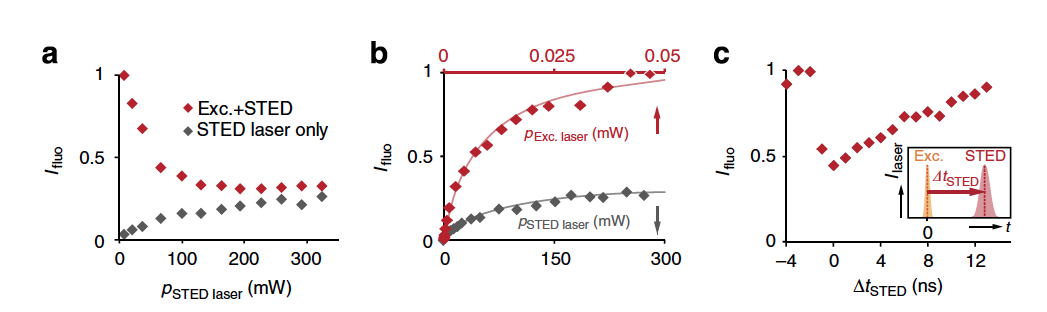
\includegraphics[width=\textwidth]{ffm23}
\end{center}

{\small За \textbf{1} взята интенсивность сигнала флуоресценции при резонансном возбуждении без применения истощения; время жизни возбужденного уровня 8 нс, диаметр 12 нм.

ВОЗБУЖДЕНИЕ: 628 нм, длина импульса 1.2 пс, частота повторений 3.8 МГц

STED: 775 нм, длина импульса 1.2 нс, частота повторений синхронизована на максимум подавления

Видим, что STED также возбуждает флуоресценцию, этот процесс является паразитным, но его сечение на несолько порядков меньше, а насыщение наступает при значительно бльшей мощности.

Отсутствие падения интенсивности при отрицательной задержке показывает, что происходит действительно STED-процесс.}

\end{frame}
\begin{frame}{Сравнение с результатами конфокальной микроскопии}
\begin{center}
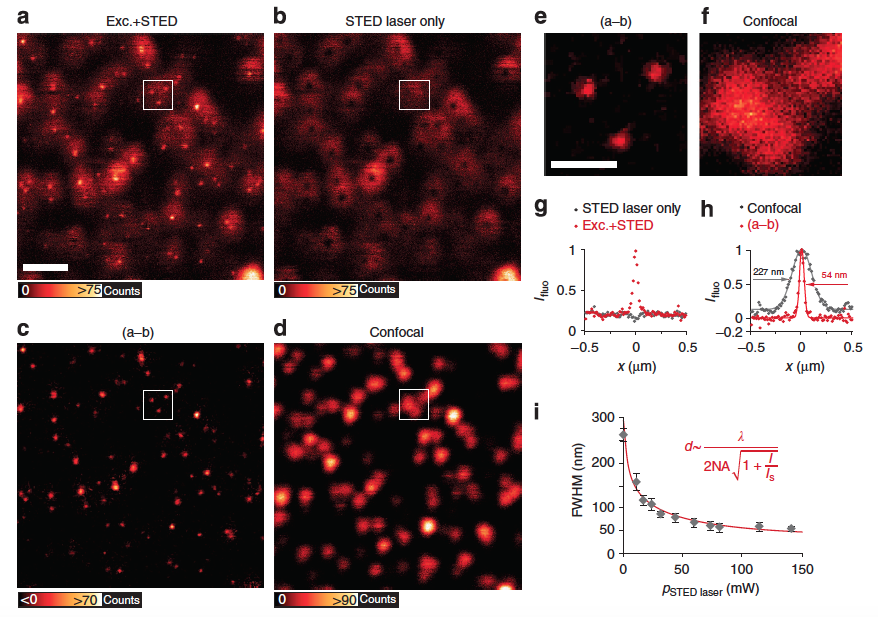
\includegraphics[width=0.9\textwidth]{ffm24}

Для того чтобы убрать гало, проиводится повторный обход только STED-лучом и затем полученное изображение вычитается из исходного.

\end{center}
\end{frame}


\begin{frame}{Подкрашивание квантовыми точками биообъектов}
\begin{center}

По методу иммунофлуоресценции подкрашены волокна виментина
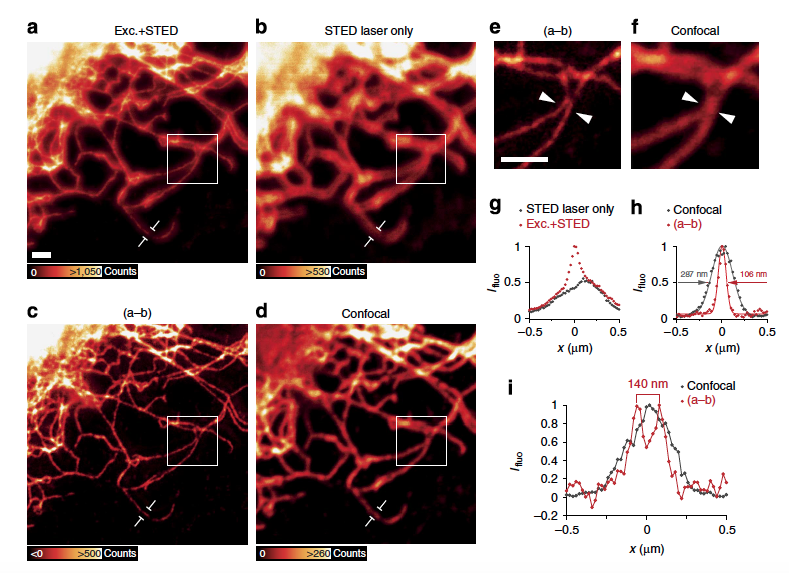
\includegraphics[width=0.9\textwidth]{ffm25}
\end{center}
\end{frame}


\begin{frame}{Выгорание квантовых точек}
\begin{center}
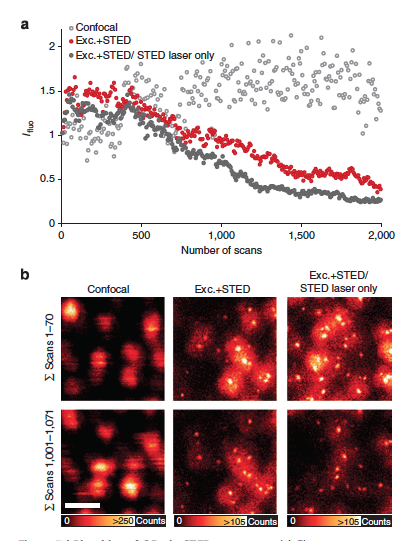
\includegraphics[width=0.6\textwidth]{ffm26}
\end{center}
\end{frame}


\begin{frame}{RESOLFT и GSD}

{\small \textcolor{red!50!black}{\textbf{GSD}} - истощение основного состояния $S_0$. Можно, оставив основной принцип STED, предложить альтернативу. Мы гасим молекулы, находящиеся на периферии фокального пятна, переводя их из возбужденного состояния $S_1$ в основное $S_0$. Вопрос в том, какая доля молекул на периферии переходит в возбужденное состояние, ведь поле на периферии значительно меньше, чем в центре? Альтернативой, в случае если невозбужденных все же остается больше, может стать истощение уровеня $S_0$. Правда, в таком случае возникает еще один вопрос. Какова должна быть скорость сканирования луча, для того, чтобы молекулы, которые мы погасили, вернулись в состояние $S_0$, в момент, когда придет их очередь быть в центре фокального пятна.}

{\small \textcolor{red!50!black}{\textbf{RESOLFT}} - reversible saturable optical fluorescence transitions microscopy - представляет из себя обощение упомянутых методик. Пусть у входящих в систему частиц есть два энергетических состояния: \textbf{A} и \textbf{B}. Природа этой разности энергий может быть любой: колебательные уровни, состояния, связывающие процессы изомеризации, и др. Главное, чтобы переход $A\rightarrow B$ был светоиндуцируемым. При этом на переход $B\rightarrow A$ мы такое требование не накладываем, он может вызываться теплом и др. Тогда:}
\begin{equation*}
\Delta x \approx \lambda/(2n \sin \alpha \sqrt{1+P/P_{sat}})
\end{equation*}

\end{frame}

\end{document}


\begin{frame}{}
\begin{columns}[c]
\column{6.5cm}
\begin{center}
\includegraphics[width=0.9\textwidth]{}
\end{center}
\column{6.5cm}
\begin{center}
\includegraphics[width=0.9\textwidth]{}
\end{center}
\end{columns}
\end{frame}

\begin{frame}{}
\begin{center}
\includegraphics[width=0.9\textwidth]{}
\end{center}
\end{frame}